\documentclass[a4paper,12pt,oneside]{book}
\usepackage{tgtermes} % times font
\usepackage{float}
\usepackage{tabularx}
\usepackage{setspace}
\usepackage{tikz}
\usepackage{xcolor}
\usepackage{pdfpages}
\usepackage{array}
\usepackage{multirow}
\usepackage{rotating}
\usepackage{colortbl} 
\usetikzlibrary{shapes, arrows, positioning}

% Define custom color for hyperlinks
\definecolor{mylinkcolor}{RGB}{0, 0, 255} % blue colored link 
\definecolor{toclinkcolor}{RGB}{0, 0, 0} % Black for Table of Contents


\usepackage{times} % Times new roman font asked in the guideline
%%%%%%%%%%%%%%% Maths symbols %%%%%%%%%%%%%%
\usepackage{amsfonts}
\usepackage{amsmath}
\usepackage{amsthm}
\usepackage{amssymb}
%\usepackage{siunitx}
%%%%%%%%%%%%%%%%%%%% Figures, tables and captions %%%%%%%%
\usepackage{graphicx}
%\usepackage{lscape}
\usepackage{caption} % Changes font of captions by putting [font=sf] before {caption} if required.
%\usepackage{dpfloat} % Ability to place figure on even or odd page using \begin{leftfullpage}
\usepackage{booktabs}
\usepackage{longtable} %for list of acronyms
\usepackage{threeparttable}
\usepackage{subcaption}

\usepackage{algorithmic}
\usepackage{textcomp}
\usepackage{multicol}
\usepackage{multirow}
\usepackage{interval}
\usepackage{adjustbox}
%%%%%%%%%%%%%%%%%%%%%% Track review changes %%%%%%%%%%%%%%%
%\usepackage{xcolor}
%\newcommand{\RV}[1]{\textcolor{violet}{#1}}

%%%%%%%%%%%%%%%%%% Numbering lines in verbatim %%%%%%%%%%%%
%\usepackage{fancyvrb}
%%%%%%%%%%%%%%%%%%%%%%%% Appendices %%%%%%%%%%%%%%%%%%%
\usepackage{appendix}

\DeclareCaptionFormat{custom}
{%
    \textbf{#1#2} #3
}
\captionsetup{format=custom}
%%%%%%%%%%%%%%%%%%%%%%%%%% Navigation %%%%%%%%%%%%%%%%%%%
% \usepackage[hidelinks,colorlinks,allcolors=blue]{hyperref} %soft-copy with color hyperlinks
\usepackage[hidelinks]{hyperref} %hard-copy no color hyperlinks

\renewcommand{\sectionautorefname}{Section}	%captitalize first s in Section while using autoref
\renewcommand{\subsectionautorefname}{Subsection}
\renewcommand{\chapterautorefname}{Chapter}
\renewcommand{\itemautorefname}{Item}
\usepackage{bookmark}	%to use startatroot feature
\newcommand*{\fullref}[1]{\hyperref[{#1}]{\autoref*{#1} \nameref*{#1}}} %navigating titles along with numbers


\usepackage[dashed=false, backend=biber, style=ieee, natbib=true, maxcitenames=2, mincitenames=1, defernumbers=true]{biblatex} %% use this for IEEE citation
\usepackage{csquotes}
\bibliography{references}
\setcounter{biburlnumpenalty}{7000} %to break DOI having strings of numbers
\usepackage[nospacearound]{extdash} %break already dashed word Otolaryngology in a reference

%%%%%%%%%%%%%% Aesthetic, control of margins, headers, etc. %%%%%%%%%%%%%%%
\usepackage{geometry}
\geometry{
left=30mm,
top=30mm,
right=25mm,
bottom=25mm
}
\setlength{\headheight}{14.49998pt} % fancyhdr need space on top
\usepackage{fancyhdr,layout}
\usepackage{etoolbox}		%to use appto command
%\oddsidemargin 1.6 cm
%\evensidemargin 0.4 cm
\pagestyle{fancy}
\renewcommand{\chaptermark}[1]{\markboth{\MakeUppercase{\chaptername}\ \thechapter.\ #1}{}}		%changing the chaptermark
%\renewcommand{\sectionmark}[1]{\markright{\thesection\ #1}} %not used
\fancypagestyle{main}{%		%pagestyles for mainmatter
\fancyhf{}
% \fancyhead[LE,RO]{\bfseries\thepage}	%page number at HeaderCenter for both even and odd pages % if I make it for two-sided book-like printing
\fancyhead[R]{\bfseries\thepage}	%page number at HeaderCenter for both even and 
\renewcommand{\headrulewidth}{0pt}	%width of the header rule
\renewcommand{\footrulewidth}{0pt}
}
%\addtolength{\headheight}{14.5pt}
\setlength{\footskip}{0in}
\renewcommand{\footruleskip}{0pt}
\fancypagestyle{plain}{%		%redefining plain page style for first few pages
\fancyhf{}
% \fancyhead[LE,RO]{\bfseries\thepage} % if I make it for two-sided book-like printing
\fancyhead[R]{\bfseries\thepage} % If I make it for single-sided printing
\renewcommand{\headrulewidth}{0pt}
}
\appto\frontmatter{\pagestyle{plain}}
\appto\mainmatter{\pagestyle{main}}
%%%%%%%%%%%%%%%%%%%%%%%%%%% Others %%%%%%%%%%%%%%%%%%%%%
\usepackage{enumerate}
\usepackage{array}	%to use arraybackslash in table
\usepackage{calc}		%to add two length variable
%\usepackage{anyfontsize}

%%%%%%%%%%%%%%%%%%%%%% Control of chapter/section headings according to the guidelines %%%%%%%%%%%%%%%%%%%%%
\usepackage[explicit]{titlesec}


\renewcommand{\thechapter}{\Roman{chapter}}
\renewcommand{\thesection}{\arabic{chapter}.\arabic{section}}
\renewcommand{\thefigure}{\arabic{figure}}
\renewcommand{\thetable}{\arabic{table}}
\renewcommand{\theequation}{\arabic{chapter}.\arabic{equation}}

\titleformat{\chapter}[display]{\normalfont\bfseries\filcenter}{\MakeUppercase\chaptertitlename\  \thechapter}{40pt}{{#1}}	%The space after the CHAPTER

\titlespacing*{\chapter} {0pt}{-30pt}{40pt} % slightly changed to look better

\titleformat{\section}{\normalfont\bfseries}{\thesection}{0.65em}{#1}
%\titlespacing*{\section}{0pt}{24pt}{12pt} 
\titlespacing*{\section} {0pt}{3.5ex plus 1ex minus .2ex}{1ex plus .2ex}	

\titleformat{\subsection}{\normalfont\bfseries}{\thesubsection}{0.65em}{#1}
%\titlespacing*{\subsection}{0pt}{20pt}{10pt}
\titlespacing*{\subsection} {0pt}{3.25ex plus 1ex minus .2ex}{.5ex plus .2ex}

\titleformat{\subsubsection}{\normalfont\bfseries}{\thesubsubsection}{0.65em}{#1}
\titlespacing*{\subsubsection}{0pt}{3.25ex plus 1ex minus .2ex}{.5ex plus .2ex}

%standard spacings from titlesec doc
% \titlespacing*{\chapter} {0pt}{50pt}{40pt}
% \titlespacing*{\section} {0pt}{3.5ex plus 1ex minus .2ex}{2.3ex plus .2ex}
% \titlespacing*{\subsection} {0pt}{3.25ex plus 1ex minus .2ex}{1.5ex plus .2ex}
% \titlespacing*{\subsubsection}{0pt}{3.25ex plus 1ex minus .2ex}{1.5ex plus .2ex}
% \titlespacing*{\paragraph} {0pt}{3.25ex plus 1ex minus .2ex}{1em}
% \titlespacing*{\subparagraph} {\parindent}{3.25ex plus 1ex minus .2ex}{1em}

%%%%%%%%%%%%%%%%%%%%%%% Line Spacing %%%%%%%%%%%%%%%%%%
% spacing 1.5
%\linespread{1.5} 
%\renewcommand{\baselinestretch}{1.5}		%controlling linespacing using baselinestretch changing, similar to the linespread command. It changes the spacing for everything in the document, including footnotes and tables
%\newcommand{\spacingR}[1]{\linespread{#1}\selectfont}		%different line spacing within the document if line spread is used
\usepackage{setspace}
%\captionsetup{font={stretch=1.5}}	%to address: setspace doesn't change the figure/table captions
\setstretch{1.5}	%onehalfspacing of LaTeX doesn't match with MS Word's 1.5 spacing, so tuned this value. Probably MS Word's 1.5 spacing is equivalent to (slightly less than) double spacing in LaTeX
%\onehalfspacing
%%%%%%%%%%%%% control the style of toc, lof, lot %%%%%%%%%%%%%%%%
\usepackage{tocloft} 
%making toc centered
\renewcommand{\cfttoctitlefont}{\hfill\large\bfseries}
\renewcommand{\cftaftertoctitle}{\hfill} 
\addtocontents{toc}{~\hfill\textbf{Page}\par}	%to pring the word "Page" above the page numbers
%making lot centered
\renewcommand{\cftlottitlefont}{\hfill\large\bfseries\MakeUppercase}
\renewcommand{\cftafterlottitle}{\hfill} 
%making lof centered
\renewcommand{\cftloftitlefont}{\hfill\large\bfseries\MakeUppercase}
\renewcommand{\cftafterloftitle}{\hfill} 

\renewcommand{\cftpnumalign}{c} %center align the page numbers
\cftsetpnumwidth{1.9em}	%so that the alighment looks good with the title "Page"
%write CHAPTER in front of chapter
\renewcommand{\cftchapfont}{}		%removing boldface
\renewcommand{\cftchappagefont}{} 	%removing boldface from page numbers
\renewcommand{\cftchappresnum}{\bfseries CHAPTER } 
\renewcommand{\cftchapaftersnum}{\quad}	%some space after chapter number
\newlength{\mylen} % a "scratch" length
\settowidth{\mylen}{\bfseries\cftchappresnum\cftchapaftersnum} % extra space
\addtolength{\cftchapnumwidth}{\mylen} % add the extra space

\cftsetindents{section}{\cftchapnumwidth}{\cftsecnumwidth} %pushing extra indent to put right below chapter title. Extra indents equal already calculated extra space (i.e., cftchapnumwidth) created by "CHAPTER " word. Section numwidth default value as cftsecnumwidth kept unaltered.
\newlength{\mysecondlen}
\setlength{\mysecondlen}{\cftchapnumwidth+\cftsecnumwidth} %subsection indent=chapter numwidth plus section numwidth
\cftsetindents{subsection}{\mysecondlen}{\cftsubsecnumwidth} %indentation for subsection just like section

% as per guideline, no dots linking to page number
\renewcommand{\cftsecdotsep}{\cftnodots} %section
\renewcommand{\cftsubsecdotsep}{\cftnodots} %subsection
\renewcommand{\cftfigdotsep}{\cftnodots} %figure; looks weird for multi-line captions
\renewcommand{\cfttabdotsep}{\cftnodots} %table; looks weird for multi-line captions

%formatting frontmatter contents
\renewcommand{\cftpartfont}{}		%removing boldface
\renewcommand{\cftpartpagefont}{\normalfont} 	%removing boldface from page numbers and giving normalfont
\setlength{\cftbeforepartskip}{1.5mm} %reducing vertical space in front matters of contents
\cftsetindents{part}{3em}{\cftpartnumwidth} %extra indentation as per guideline

%%%%%%%%%%%%%%%%%%%%%% Paragraph Indentation %%%%%%%%%%%%%%%
\usepackage{parskip}	%to have a vartical space instead of indentation in paragraph... as per guideline. It has a slight clash with the tocloft package; suggested to declare after toclof % the packages and their settings in a separate file

% Set hyperlink color globally
\hypersetup{
  colorlinks=true,
  linkcolor=mylinkcolor,
  citecolor=mylinkcolor,
  urlcolor=mylinkcolor,
}

%%%%%%%%%%%%%%%%%%%% Some new custom commands %%%%%%%%%%%%%%%%%
\newcommand{\blanklineR}{\hfill \\} %to have blanklines
\newcommand{\HeadingR}[1]{
{\large		
\bfseries{#1}}}
\newcommand{\titleR}{Power Quality Issues of Smart Grid Technology: Routing System 
Adaptability through Statistics and Forecasts} 

%%%%%%%%%%%%%%%%% PDF meta-data %%%%%%%%%%%%%%%%%%%%%%%%
\hypersetup{%
pdfauthor={Md. Ohiduzzaman Sajol and Sadman Shamyo},
pdftitle=\titleR,
pdfsubject={EE-3122 Project Report},
pdfkeywords={}
}
%%%%%%%%%%%%%%%%%%%%%%%%%%%%%%%%%%%%%%%%%%%%%%%%%%%%%%%%%%%%%%%%%%%%%%%%%%%%%%%%%%%%%%%%%%%%
%%%%%%%%%%%%%%%%%%%%%%%%%%%% DOCUMENT STARTS %%%%%%%%%%%%%%%%%%%%%%%%%%%%%%%%%%%%%%%%%%%%%%%%%%%
%%%%%%%%%%%%%%%%%%%%%%%%%%%%%%%%%%%%%%%%%%%%%%%%%%%%%%%%%%%%%%%%%%%%%%%%%%%%%%%%%%%%%%%%%%%%
\begin{document}
\frontmatter
%%%%%%%%%%%%%%%%%%% Title Page %%%%%%%%%%%%%%%%%%%%%
\begin{titlepage}
\phantomsection
\addcontentsline{toc}{part}{Title Page}	
\centering
%\begin{onehalfspacing}
%\linespread{1.3}
\HeadingR{\MakeUppercase{\titleR}}
%\end{onehalfspacing}\\
\blanklineR\blanklineR\blanklineR
{\fontsize{16}{12}\selectfont \textbf{Submitted By:}}\\
\blanklineR
{\fontsize{14}{12}\selectfont \MakeUppercase{MD OHIDUZZAMAN SAJOL}      \hspace{1.15cm}     \MakeUppercase{ROLL NO: 2003043}}
\blanklineR
{\fontsize{14}{12}\selectfont \MakeUppercase{SADMAN SHAMYO}      \hspace{1.15cm}     \MakeUppercase{ROLL NO: 2003060}}
\blanklineR\blanklineR\blanklineR
{\fontsize{16}{12}\selectfont \textbf{Submitted To:}}\\
\blanklineR
{\fontsize{14}{12}\selectfont \MakeUppercase{Dr. MOHIUDDIN AHMED}\\
\MakeUppercase{\textit{PROFESSOR, DEPT. OF EEE, KUET}}}\\
\blanklineR
{\fontsize{14}{12}\selectfont \MakeUppercase{Dr. MD. SHAHJAHAN}\\
\MakeUppercase{\textit{PROFESSOR, DEPT. OF EEE, KUET}}}\\
\blanklineR\blanklineR\blanklineR

\includegraphics[width=0.26\textwidth]{Figures/kuet_logo.jpg}
\blanklineR\blanklineR\blanklineR
\end{titlepage}


%%%%%%%%%%%%%%%%%%%% Abstract %%%%%%%%%%%%%%%%%%%%%%%%%
\newpage
\phantomsection \label{abstr}
\addcontentsline{toc}{part}{Abstract}

\begin{center}
\HeadingR{\MakeUppercase{Abstract}}
\end{center}
Smart grid technology is a new horizon in power system engineering. It came into life with a view to ensuring reliable, safe and cost-efficient power generation, transmission and distribution. Breakthroughs in wireless communication arena have fortified the implementation of smart grid networking system in different countries. In Bangladesh, this concept is almost new\cite{6497752}. As soon as the smart grid will be concrete, the power sector of Bangladesh will experience significant increase in power generation and cost reduction which will one day lead to 24/7 power supply to all houses, industries etc. Primitive power network in our country often experiences system loss, faults and wastage due to poor power quality. An important issue is to have powerful tools at hand able to measure power quality parameters in a flexible way in such grids\cite{6563537}. This study casts light on a way to determine the status of power quality in transmission lines and distributors. In addition to that, a procedure of forecasting voltage instability with linear regression is made. This is done by a machine learning algorithm.
\\\\
\textbf{Keywords:} Power quality, Voltage interruption, Multiple correlation coefficient, Linear regression, Machine learning, Smart grid, Gradient Descent, Skewness, Kurtosis.

%%%%%%%%%%%%%%%%%%% Contents %%%%%%%%%%%%%%%%%%%%%%%%%%
\newpage
\renewcommand\contentsname{CONTENTS}
\addcontentsline{toc}{part}{Contents}
\begin{singlespacing}
{\hypersetup{linkcolor=black}
\tableofcontents
}
\end{singlespacing}

%%%%%%%%%%%%%%%%%%%%%% Introduction %%%%%%%%%%%%%%%%%%%%%%%%%%%%
\chapter{INTRODUCTION}\label{chap:intro}
Generally smart grid is a modern technology of power system which can convert the whole power system in to digital format. In brief, a smart grid is the use of sensors, communications, computational ability and control in some form to enhance the overall functionality of the electric power delivery system\cite{6497752}. Power quality refers to how well electricity delivered to equipment matches the required characteristics\cite{clou2023}. Its disruptions arise system losses and even power outage. 
Aims of the project are to collect samples of power quality parameters and make statistical analysis on them alongside with time series forecasting by incentive training algorithm. All the tasks are done in python programming language and the source codes can be found in the \autoref{app:myappendix}. Measurement of dispersion indices of data will reveal the quality status of power. In order to make adaptations in power transmission and distribution system to improve quality, pre-measurement of quality situation is compulsory. The project is based on this measurement technique.
In the future, if smart grid is established in our country, power quality monitoring systems will be digitalized and will be connected to any communication media that will establish a link between PDB and consumers. A need of an intelligent software to analyze power quality will rise then. So, we have developed a prototype program that can be attached to such software.



%%%%%%%%%%%%%%%%%%%%%%%%%%%%%%%%% Methodology %%%%%%%%%%%%%%%%%%%%%%%
\newpage
\chapter{METHODOLOGY}\label{chap:method}
\label{sec:methods}

\section{A Bird's Eye View}

\begin{figure}[htp]
\centering
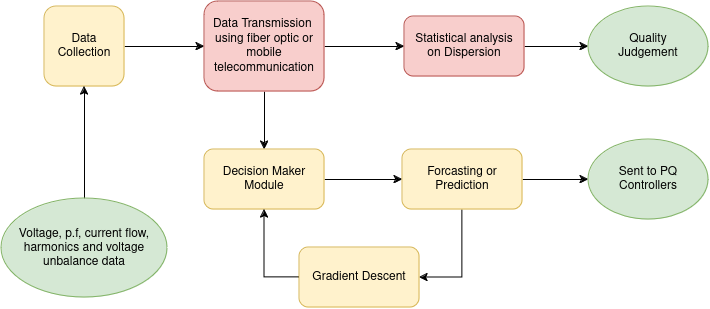
\includegraphics[width=0.9\textwidth]{Figures/flow-chart.png} 
\caption{The overall procedure of the project}
\label{fig:flowchart}
\end{figure}

\section{Statistical Analysis}
For a set of `n` numbered ungrouped data $(x_1, x_2, x_3, \ldots, x_n)$ and for $\bar{x}$ as the mean of the data,

1. Mean deviation, M.D = $\frac{1}{n}\sum_{i=1}^{n}|x_i - \bar{x}|$ \\
2. Standard deviation, $\sigma$ = $\sqrt{\frac{1}{n}\sum_{i=1}^{n}(x_i - \bar{x})^2}$\\
3. Skewness, S = $\frac{1}{n}\sum_{i=1}^{n}\left(\frac{x_i - \bar{x}}{\sigma}\right)^3$\\
4. Kurtosis, B = $\frac{1}{n}\sum_{i=1}^{n}\left(\frac{x_i - \bar{x}}{\sigma}\right)^4$

Correlation coefficient shows the balance index of current flow in three phase system. Let, $x$, $y$ and $z$ are three separate datasets. A relation can be established among three sets.

Multiple correlation coefficient, CC = $\frac{\sqrt{r_{xy}^2 + r_{yz}^2 + r_{zx}^2 - 2r_{xy}r_{yz}r_{zx}}}{\sqrt{(1-r_{xy}^2)(1-r_{yz}^2)(1-r_{zx}^2)}}$

Where, $r_{xy} = \frac{\sum_{i=1}^{n}(x_i - \bar{x})(y_i - \bar{y})}{n\sigma_x\sigma_y}$, $r_{yz} = \frac{\sum_{i=1}^{n}(y_i - \bar{y})(z_i - \bar{z})}{n\sigma_y\sigma_z}$, $r_{zx} = \frac{\sum_{i=1}^{n}(z_i - \bar{z})(x_i - \bar{x})}{n\sigma_z\sigma_x}$

\newpage
\section{Forecasting: Decision Maker Module}
\begin{figure}[htp]
\centering
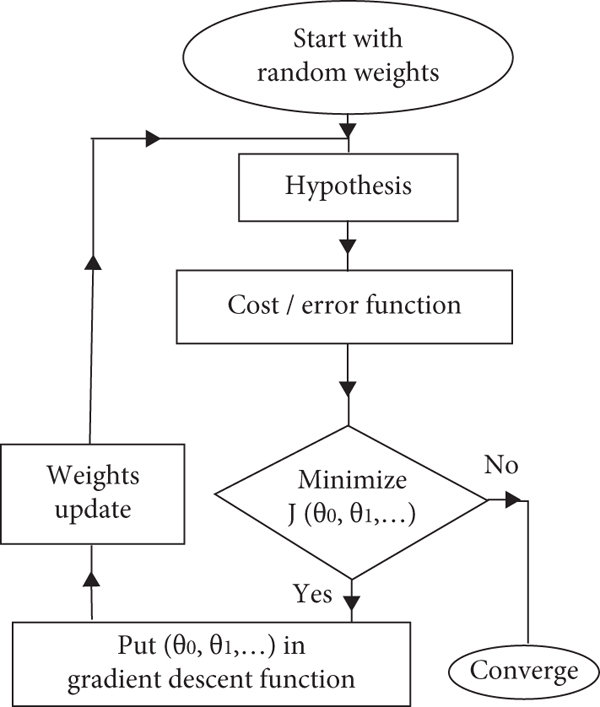
\includegraphics[height=10cm]{Figures/Flow-chart-of-linear-regression.jpg} 
\caption{The internals of the forecasting module\cite{9270536}}
\label{fig:flowchart-linear-regression}
\end{figure}

\subsection{Associated Equations}
\begin{itemize}
\item \textbf{Hypothesis function:}
\begin{equation}
h_{\theta}(X) = \theta^T X + b = \theta_0 + \theta_1 \cdot X_1 + \theta_2 \cdot X_2 + \theta_3 \cdot X_3 + \theta_4 \cdot X_4
\end{equation}

\item \textbf{Mean Squared Error (MSE) Loss function:}
\begin{equation}
J(\theta, b) = \frac{1}{2m} \sum_{i=1}^{m} (h_{\theta}(X^{(i)}) - y^{(i)})^2
\end{equation}

\item \textbf{Gradient of the Loss function with respect to weights ($\theta$) and bias ($b$):}
\begin{equation}
\frac{\partial J}{\partial \theta} = \frac{1}{m} X^T(h_{\theta}(X) - y)
\end{equation}
\begin{equation}
\frac{\partial J}{\partial b} = \frac{1}{m} \sum_{i=1}^{m} (h_{\theta}(X^{(i)}) - y^{(i)})
\end{equation}

\item \textbf{Parameter Update (Gradient Descent):}
\begin{equation}
\theta := \theta - \alpha \frac{\partial J}{\partial \theta}
\end{equation}
\begin{equation}
b := b - \alpha \frac{\partial J}{\partial b}
\end{equation}

\item \textbf{Prediction:}
\begin{equation}
y_{\text{pred}} = h_{\theta}(X)
\end{equation}

\item \textbf{Normalization of Features:}
\begin{equation}
X_{\text{normalized}} = \frac{X - X_{\text{min}}}{X_{\text{max}} - X_{\text{min}}}
\end{equation}
\end{itemize}

Here,
\begin{itemize}
\item $\theta_0 = b$ is the bias term,
\item $\theta_1$ corresponds to the weight for Power Demand, $X_1$,
\item $\theta_2$ corresponds to the weight for Month, $X_2$,
\item $\theta_3$ corresponds to the weight for Day of the Week, $X_3$,
\item $\theta_4$ corresponds to the weight for Time of the Day, $X_4$,
\item $m$ is the number of training examples.
\end{itemize}
%%%%%%%%%%%%%%%%%%%%%%%%%%%%%%%%%%%%%%%%%%%%%%%%%%%%%%%
\chapter{RESULTS} \label{chap:result}
\label{sec:results}

\section{Collection and Tabulation of Data}
Data acquisition system SEMCE DAQ is used for continuous data monitoring of electrical parameters, such as voltage, current, frequency, power, harmonics and total harmonic distortion (THD) in electrical networks\cite{6563537}. 
All the samples collected from grid system is made possible by this oscilloscope device equipped with IoT interface. This is a power analyzer tool that can monitor 3 phase system.

%-----------------------------------------------------
\begin{table}[ht]
  \centering
  \caption{Harmonic Samples of Phase Voltages\cite{6563537}}
  \begin{tabular}{|c|c|c|c|}
  \hline
  \textbf{Order} & \textbf{$V_{ab}$(\%)} & \textbf{$V_{bc}$(\%)} & \textbf{$V_{ca}$(\%)} \\
  \hline
  1 & 100 & 100 & 100 \\
  2 & 0.05 & 0.07 & 0.05 \\
  3 & 0.05 & 0.05 & 20.03 \\
  4 & 0.05 & 0.05 & 0.06 \\
  5 & 35.28 & 0.06 & 0.05 \\
  6 & 0.07 & 0.06 & 0.05 \\
  7 & 0.05 & 44.88 & 0.05 \\
  8 & 0.07 & 0.06 & 0.06 \\
  9 & 0.06 & 0.08 & 0.05 \\
  10 & 0.08 & 0.06 & 0.05 \\
  \hline
  \end{tabular}
  \label{tab:harmonic-samples-voltage}
  \end{table}



\begin{table}[ht]
  \centering
  \caption{Harmonic Samples of Phase Currents\cite{6563537}}
  \begin{tabular}{|c|c|c|c|}
  \hline
  \textbf{Order} & \textbf{$I_{a}$(\%)} & \textbf{$I_{b}$(\%)} & \textbf{$I_{c}$(\%)} \\
  \hline
  1 & 100 & 100 & 100 \\
  2 & 0.06 & 5.22 & 10.02 \\
  3 & 0.07 & 64.32 & 61.36 \\
  4 & 0.09 & 0.08 & 0.08 \\
  5 & 0.08 & 17.76 & 15.02 \\
  6 & 0.05 & 0.07 & 0.05 \\
  7 & 0.05 & 24.62 & 35.06 \\
  8 & 0.08 & 0.08 & 0.08 \\
  9 & 0.06 & 0.09 & 0.07 \\
  10 & 0.08 & 0.06 & 0.06 \\
  \hline
  \end{tabular}
  \label{tab:harmonic-samples-currents}
  \end{table}

\newpage
  \begin{table}[ht]
    \centering
    \caption{Current Samples taken over a fixed time span (Current variation scenario)\cite{THENTRAL20225370}}
    \begin{tabular}{|c|c|c|c|}
    \hline
    \textbf{Sample no.} & \textbf{$I_a$ (A)} & \textbf{$I_{b}$ (A)} & \textbf{$I_{c}$ (A)} \\
    \hline
    1 & 0.5 & 1.5 & 2 \\
    2 & 5 & 1.3 & 1.8 \\
    3 & 5.2 & 1.45 & 2.2 \\
    4 & 6.1 & 1.48 & 2.1 \\
    5 & 6.2 & 1.5 & 2.6 \\
    6 & 6.2 & 1.6 & 2.55 \\
    7 & 6.7 & 1.9 & 2.5 \\
    8 & 7.2 & 2.1 & 2.53 \\
    9 & 8 & 2.6 & 2.6 \\
    10 & 8.3 & 3.5 & 3.2 \\
    \hline
    \end{tabular}
    \label{tab:current-samples}
    \end{table}

    \begin{table}[ht]
      \centering
      \caption{Frequency samples taken over  a fixed time span\cite{8586572}}
      \begin{tabular}{|c|c|}
      \hline
      \textbf{Sample no.} & \textbf{Frequency (Hz)} \\
      \hline
      1 & 50.5 \\
      2 & 50.6 \\
      3 & 50.4 \\
      4 & 49.9 \\
      5 & 50.3 \\
      6 & 50.52 \\
      7 & 50.4 \\
      8 & 50.3 \\
      \hline
      \end{tabular}
      \label{tab:frequency-samples}
      \end{table}

      \begin{table}[h!]
        \centering
        \caption{Voltage samples taken over a fixed time span\cite{9230639}}
        \begin{tabular}{|c|c|c|}
        \hline
        \textbf{Sample no.} & \textbf{Demand} & \textbf{Line voltage} \\
        \hline
        1 & 72 & 99 \\
        2 & 66.6 & 104.016 \\
        3 & 64 & 105.6 \\
        4 & 58.6 & 108.24 \\
        5 & 55.4 & 112.2 \\
        6 & 57.6 & 109.56 \\
        7 & 60.8 & 105.6 \\
        8 & 64 & 104.28 \\
        \hline
        \end{tabular}
        \label{tab:voltage-samples}
        \end{table}

  \newpage
  \section{Statistical Analysis}
        \begin{figure}[h!]
          \centering
          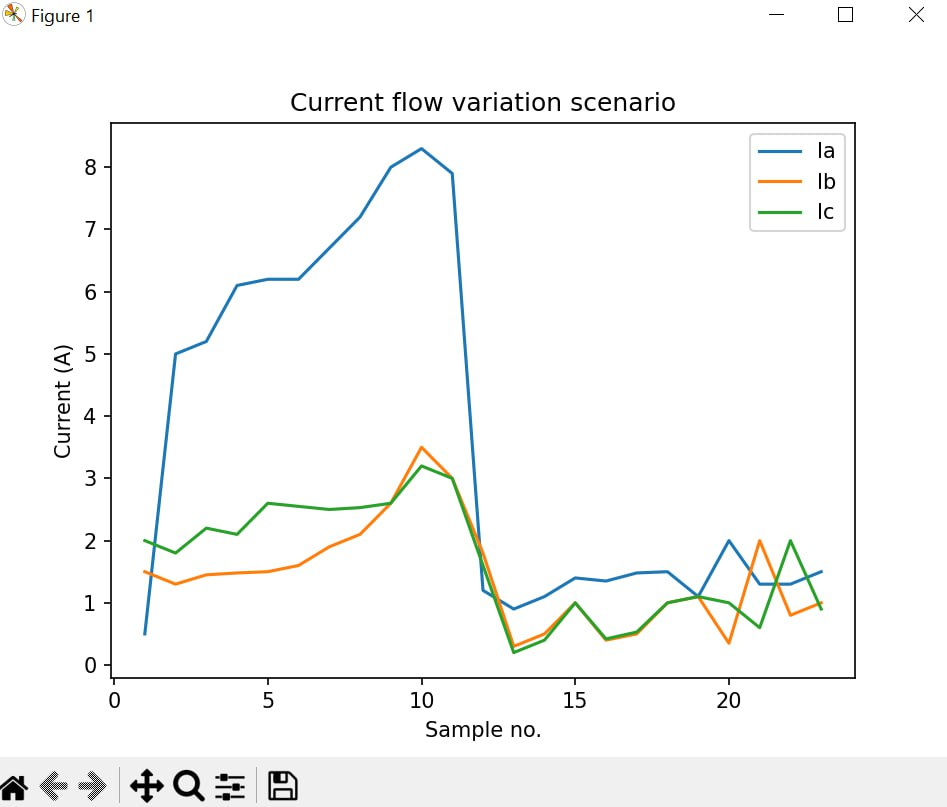
\includegraphics[height=10cm]{Figures/1.jpg} 
          \caption{Current flow variation graph(3-phase system)}
          \label{fig:current-flow-variation}
        \end{figure}

        \begin{figure}[ht]
          \centering
          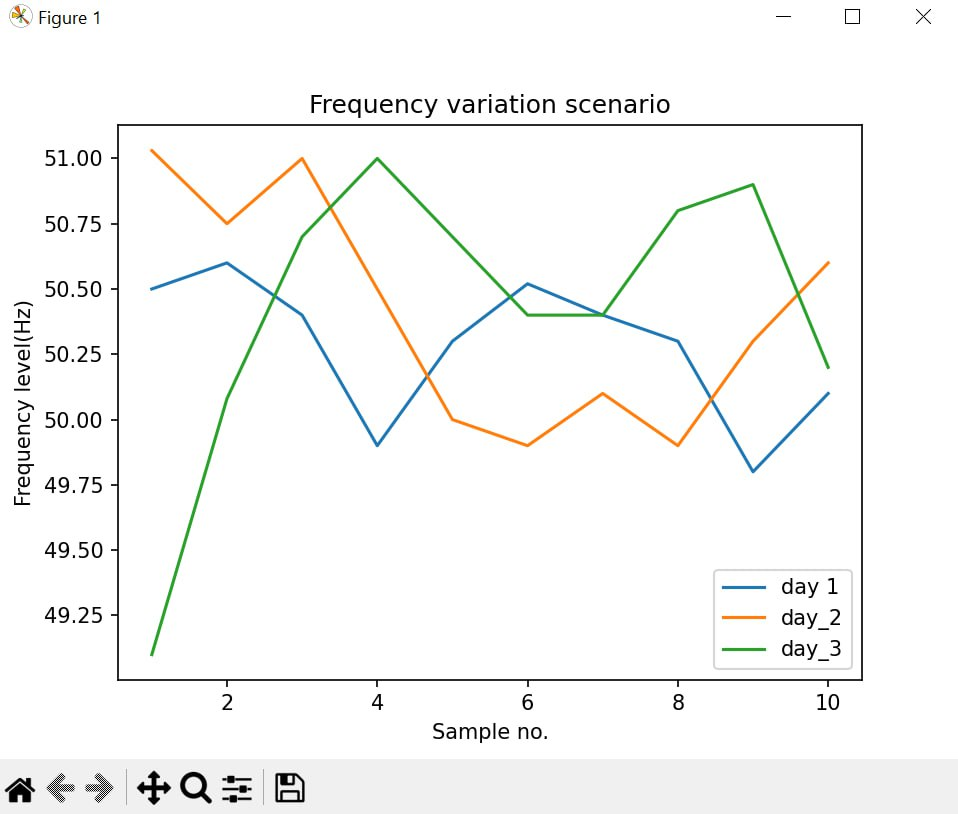
\includegraphics[height=10cm]{Figures/2.jpg} 
          \caption{Frequency scenario over three days in transmission line.}
          \label{fig:Frequency-scenario}
        \end{figure}


\begin{table}[h!]
  \centering
  \caption{Data obtained from frequency fluctuation level monitoring module}
  \begin{tabular}{|c|c|c|c|c|}
  \hline
  \textbf{Day no.} & \textbf{Mean Deviation} & \textbf{Standard Deviation} & \textbf{Skewness} & \textbf{Kurtosis} \\
  \hline
  1 & 0.2 & 0.06 & 3.16 & 9.99 \\
  2 & 0.368 & 0.06 & 3.16 & 10 \\
  3 & 0.392 & 0.072 & 3.16 & 10 \\
  \hline
  \end{tabular}
  \label{tab:frequency-fluctuation}
  \end{table}

  Correlation Coefficient of three phase current magnitude = 0.889\\
  Correlation Coefficient of voltage harmonics = 0.936\\
  Correlation Coefficient of current harmonics = 0.993

  \newpage
  \begin{figure}[h!]
    \centering
    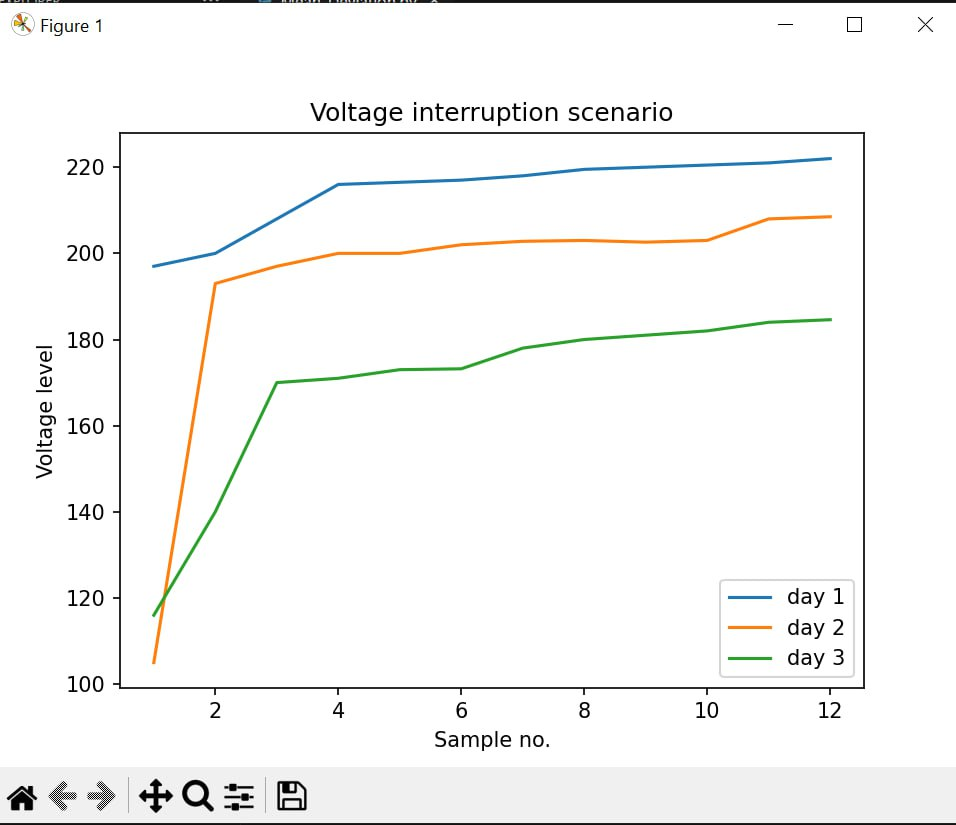
\includegraphics[height=10cm]{Figures/3.jpg} 
    \caption{Voltage interruptions in three consecutive days}
    \label{fig:voltage-interruptions}
  \end{figure}

  \newpage
  \begin{figure}[h!]
    \centering
    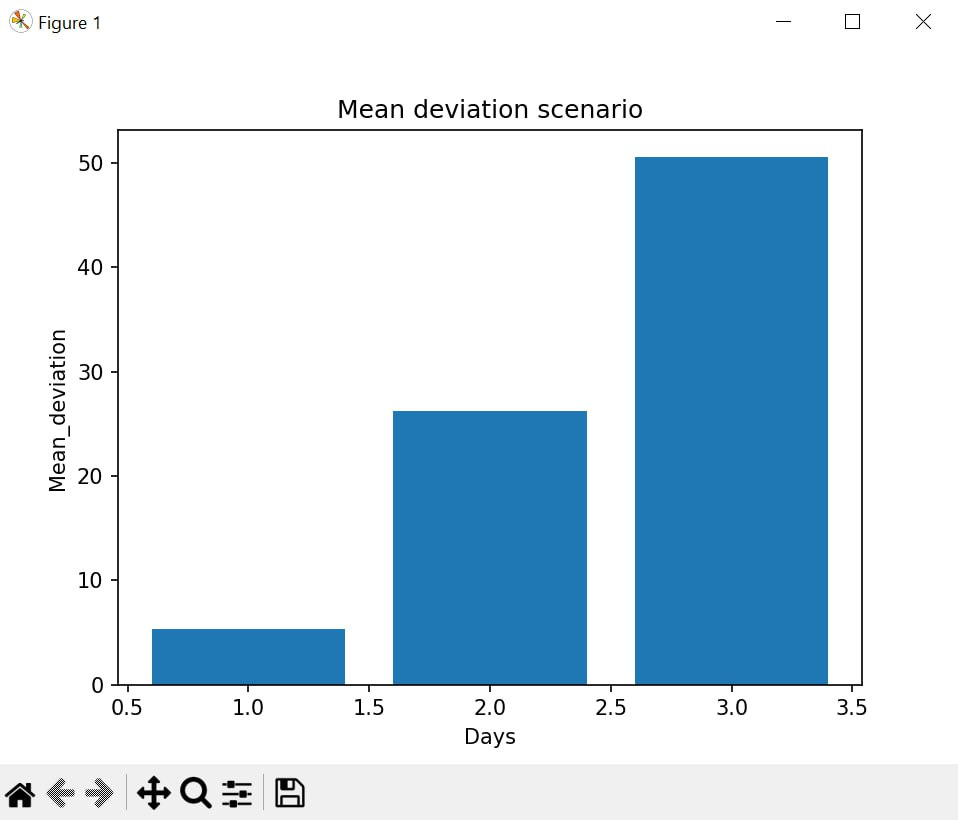
\includegraphics[height=10cm]{Figures/4.jpg} 
    \caption{Mean deviation of voltage interruption}
    \label{fig:mean-deviation}
  \end{figure}

  \begin{figure}[h!]
    \centering
    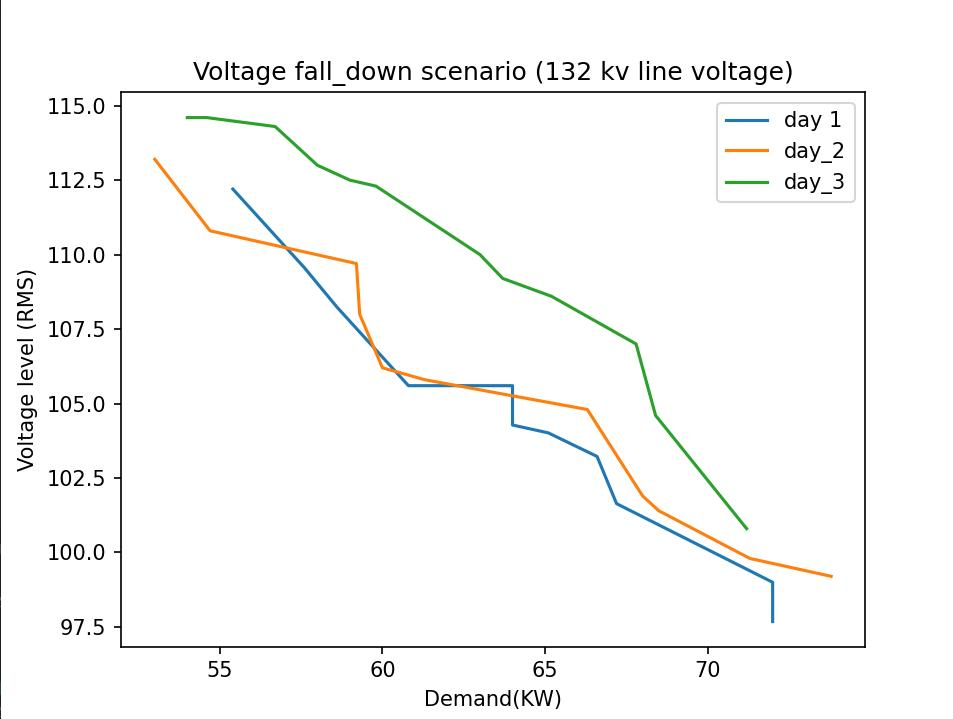
\includegraphics[height=10cm]{Figures/5.jpg} 
    \caption{Voltage Fall down scenario for 132kV line voltage.}
    \label{fig:voltage-drops}
      \end{figure}

%-----------------------------------------------------------------------------
\newpage\newpage\newpage
    % \section{Decision Making with Machine Learning}
  \section{Simulated data and Prediction for Voltage Unbalance}
  \begin{figure}[h!]
    \centering
    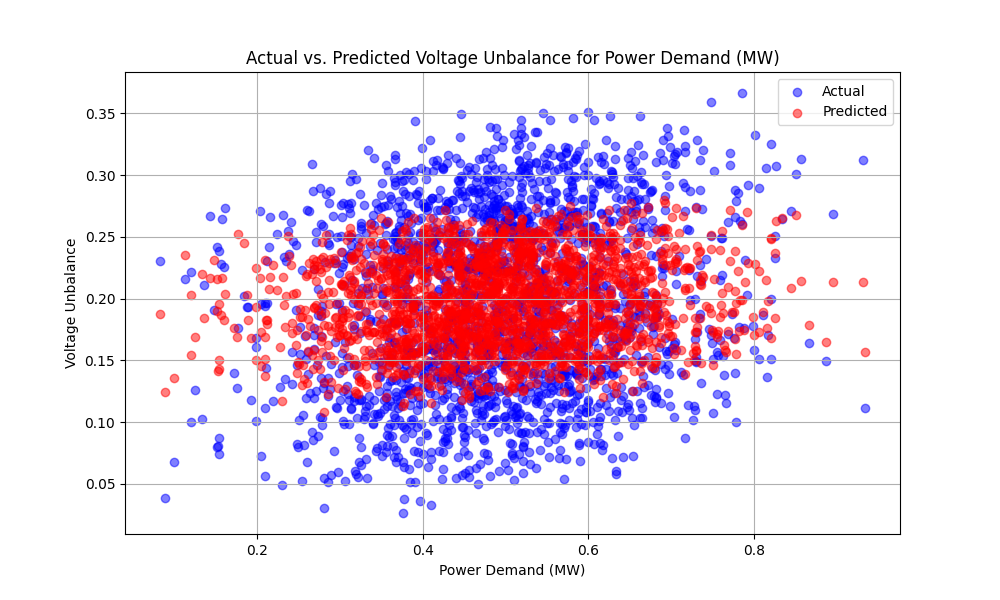
\includegraphics[height=10cm]{Figures/predicted_data/Actual vs. Predicted Voltage Unbalance for Power Demand (MW).png} 
    \caption{Actual vs. Predicted Voltage unbalance for Power Demand(MW)(see \autoref{app:myappendix})}
    \label{fig:voltage-drops}
  \end{figure}

  
  \begin{figure}[h!]
    \centering
    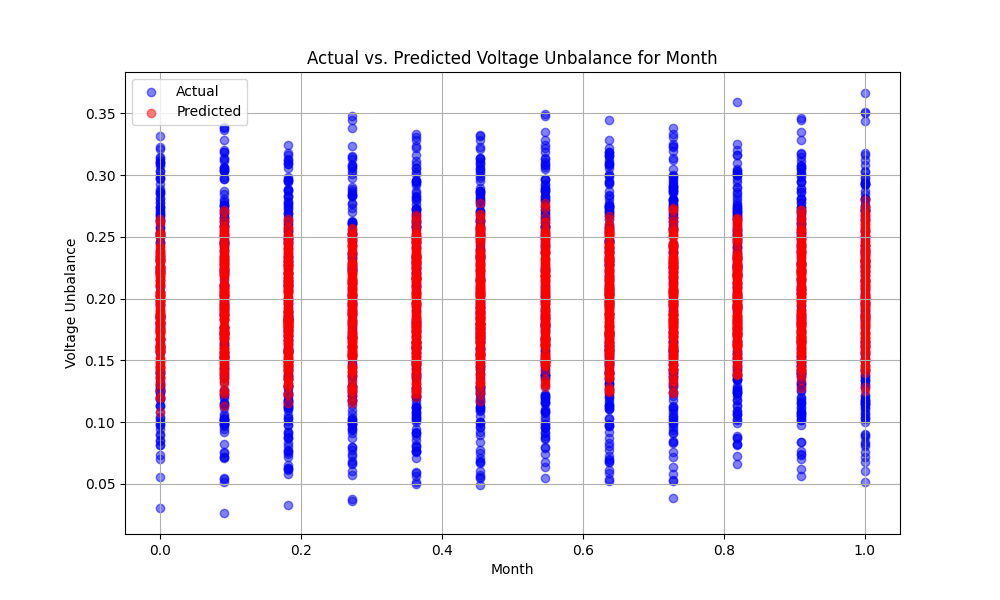
\includegraphics[height=10cm]{Figures/predicted_data/Actual vs. Predicted Voltage Unbalance for Month.png} 
    \caption{Actual vs. Predicted Voltage Unbalance for Month.(see \autoref{app:myappendix})}
    \label{fig:voltage-drops}
  \end{figure}


  \begin{figure}[ht]
    \centering
    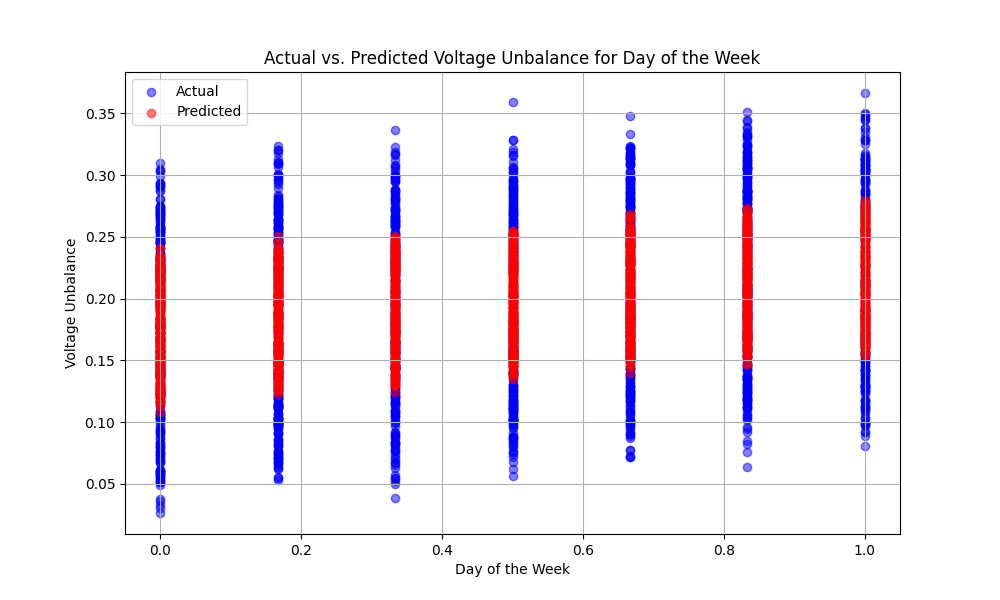
\includegraphics[height=10cm]{Figures/predicted_data/Actual vs. Predicted Voltage Unbalance for Day of the Week.png} 
    \caption{Actual Vs. Predicted Voltage Unbalance for the day of the week.(see \autoref{app:myappendix})}
    \label{fig:voltage-drops}
  \end{figure}


  \begin{figure}[ht]
    \centering
    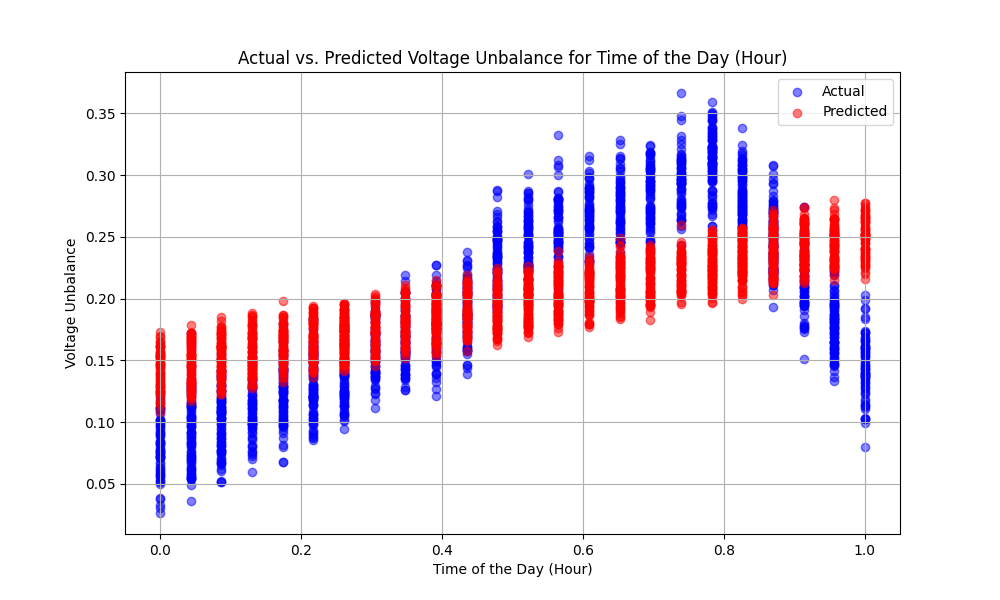
\includegraphics[height=10cm]{Figures/predicted_data/Actual vs. Predicted Voltage Unbalance for Time of the Day (Hour).png} 
    \caption{Actual Vs. Predicted voltage unbalance for Time of the Day (Hour)(see \autoref{app:myappendix})}
    \label{fig:voltage-drops}
  \end{figure}




%%%%%%%%%%%%%%%%%%%%%%%%%%%%%%%%%%%%%%%%%%%%%%%%%%%%%%%
\chapter{DISCUSSIONS} \label{chap:disc}
\label{sec:discussion}

\section*{Quality Analyzer Module}
The estimations of dispersive nature of the factors inhibiting power quality aided in determining the quality index.\\
The MD and standard SD virtually gives an idea of error level. An increased magnitude of MD and SD will indicate poor performance of power system. For example: High SD of voltage level indicates poor voltage regulation of generation system.  In the experiment mean deviation of voltage is between 3.42 and 3.52, which  means that regulation of system is fair. The SD too is less than 1. If somehow regulation falls, the information hub will inform the relevant generation station. The governor of alternator will make necessary decisions then.\\
Skewness and Kurtosis provide an insight of data density at edges. The equivalent result of skewness and kurtosis of voltage and frequency shows that their increment and decrement is same and symmetrical. This will generate a data density profile that takes the shape of uniform hill.\\
The CC of three phase current indicates the balance factor. High CC will mean that the magnitude of all three phase currents is almost same. As it is known that at household level, the power factor of all phases remains fairly same, only the magnitude of current will unveil any unbalanced system. Unbalanced three phase current cause neutral wire to carry current. If balance factor is less (indicated by CC), then unbalancing will be more and neutral wire will be more subjected to wear and tear. The CC of three phase current is 0.889 which tells that balance index is not good. If  there is a phase fault, the CC will reduce sharply. The controllers at distributors will get informed about this and will bring actions.\\
The CC of harmonics is needed to update the active harmonic filters at distribution substations. The work distribution among the filters installed at each phase will be dictated by CC of harmonics of Line voltages.
\newpage
\section*{Decision Maker Module}
The Decision Maker Module can make future prediction from present or past power demand taking into account the probable effect of when the prediction is being made and gives the probable unbalance level which can be used to adapt with the situation to ensure maximum PQ.\\
Its job is not only to make predictive decision but also collect data and evaluate itself with the collected data and from the evaluation updates its parameters so that in future in similar scenarios it can make more appropriate decisions.\\
From the data, it's evident that the module can learn the trend up to the point when Unbalance level is maximum, learning rate after that of is poor. This may have been improved by choosing a nonlinear model.


%%%%%%%%%%%%%%%%%%%%%%%%%%%%%%%%%%%%%%%%%%%%%%%%%%%%%%%%%%%%%%%%%%%%%%%%%%%%%
\chapter{CONCLUSIONS}\label{chap:concl}
\label{sec:conclusion}
Power quality monitoring and adjustment of disruptions is much needed fairly reliable power generation, distribution and transmission system. Smart grid has indeed come with the idea of real time data sampling form various ends of power system.\\
According to the Recent ‘Power System Master Plan’ by BPDB (Bangladesh Power Development Board) the transmission loss will be reduced to 3\% by 2018 and distribution loss will be reduced to 10\% by 2019. But it may be not possible due to some hurdles like- corruption, insufficient technological support and political uncertainty. In that case smart grid technology can be a good choice.\\
This study has remarked on the power status and forecasted voltage unbalance with demand that will help in smooth operation of smart grid system.

\backmatter
\renewcommand\bibname{REFERENCES}
\phantomsection \label{refs}
\addcontentsline{toc}{part}{REFERENCES}
\printbibliography[title={REFERENCES}]


\appendix
\chapter{\MakeUppercase{Appendices}}
\label{app:myappendix}
\addcontentsline{toc}{part}{\MakeUppercase{APPENDICES}}
\section*{Data and Code availability}
All the \href{https://github.com/ohid-sajol/Project-On-EE-3122-Numerical-Methods-And-Statistics/blob/main/simulated_voltage_unbalance_data.csv}{data}, \href{https://github.com/ohid-sajol/Project-On-EE-3122-Numerical-Methods-And-Statistics/blob/main/simulated_data_generator.ipynb}{data simulator}, \href{https://github.com/ohid-sajol/Project-On-EE-3122-Numerical-Methods-And-Statistics/blob/main/Linear_Regressor.ipynb}{code} and other necessary files associated with this project can be found in this repository:\\ \href{https://github.com/ohid-sajol/Project-On-EE-3122-Numerical-Methods-And-Statistics}{https://github.com/ohid-sajol/Project-On-EE-3122-Numerical-Methods-And-Statistics}
\end{document}


